%#! platex %f && dvipdfmx -d 5 tougetsuan180205a
%
%
% 手で,コンパイルする方法
% platex tougetsuan180205a
% pbibtex tougetsuan180205a
% platex tougetsuan180205a
% dvipdfmx -d 5 tougetsuan180205a
%
\documentclass[a4paper,twocolumn,twoside,10pt]{jarticle}
\usepackage{nidanfloat} %% add
\usepackage{graphics}
\usepackage[dvips,usenames]{color}  % for revise color
\usepackage{graphicx}
\usepackage{plain}
\usepackage{fancyhdr}
\pagestyle{fancyplain}
\usepackage{amssymb}
\usepackage{bm}
\usepackage{float}
%フロート環境とその前後の本文とのスペース
\setlength\floatsep{0pt} %ページ上部あるいは下部に出力されるフロートとフロートの間の距離
\setlength\intextsep{8pt} %ページの途中に出力されるフロートとその前後の本文との距離
%\setlength\textfloatsep{0pt} %ページ上部のフロートと本文,および本文と
%ページ下部のフロートとの距離
\setcounter{page}{13}
\topmargin = -15mm
\oddsidemargin = 0mm
\evensidemargin = -10mm
\textwidth = 162mm
\textheight = 250mm
\columnsep = 10mm
\renewcommand{\footrulewidth}{0pt}
\renewcommand{\headrulewidth}{0pt}
\bmdefine{\bx}{x}



\begin{document}
\lhead{}
\rhead{}
%\rhead{2014年2月13日}
% \begin{twocolumn}
\twocolumn[
\begin{center}
{\Large
神経回路モデルによる....}
\vspace{3mm}  \\
{\large 宮崎大学 工学部 情報システム工学科}\vspace{2mm} \\
{\large 67140770  桃月庵 あられ} \vspace{10mm}\\
\end{center}]

%\input{titles}
\section{$B$O$8$a$K(B}
$BH82H$K$O!$8E:#Db;V$sD+$dLx2H>.;0<#$N$h$&$K(B
$BL>?M$H8F$P$l$k?M$,B8:_$9$k(B\cite{amari89a}$B!%(B
$BL>?M$O!$$[$+$NH82H$H$I$3$,0c$&$N$@$m$&!%(B
$B$?$H$($P!VAF9zD920!W$H$$$&OC!%(B
$B$$$m$$$m$JH82H$,1i$8$k$,!$1i<T$K$h$C$FLLGr$5$,0[$J$k!%(B
$BF1$8OC$G$"$k$N$K!$$3$l$O$J$<$@$m$&(B
$B!J"($3$s$JLLGr$$LdBj$,$"$k!K!%(B
$B!J$=$NLdBj$KBP$7$F$3$l$^$G$I$s$J8&5f$,$J$5$l$F$-$?$+!$8&5f$NNr;K$rDI$&!K!%(B
$B!J$^$@8&5f$OIT==J,!%$3$NE@$,J,$+$C$F$$$J$$!%$3$l$,2r7h$G$-$l$P!*!K!%(B
$B$=$NLdBj$r2r7h$9$k$?$a!$K\O@J8$G$O(B.........$B<B83$r$*$3$J$C$?!%(B
$B$=$N7k2L!$(B... $B$G$"$k$3$H$,J,$+$C$?!%$3$l$O(B....$B$r0UL#$9$k!%(B


  % はじめに
\section{$B?@7P2sO)%b%G%k$H3X=,<jK!(B}
$B$3$3$O<jK!!%(B

\subsection{$B8m:95UEAGEK!(B}
$B%9%Z!<%9$NET9g>e!$@bL@$O>JN,$9$k!%(B
  % 手法
%\rhead{}
%\input{experiment}  % 実験
\section{結果}
% --- experiment.tex から移動 ここから
\subsection{一層目の重みの学習}
\begin{figure}[hbt]
\centering
\begin{minipage}{0.45\columnwidth}
  \centering
  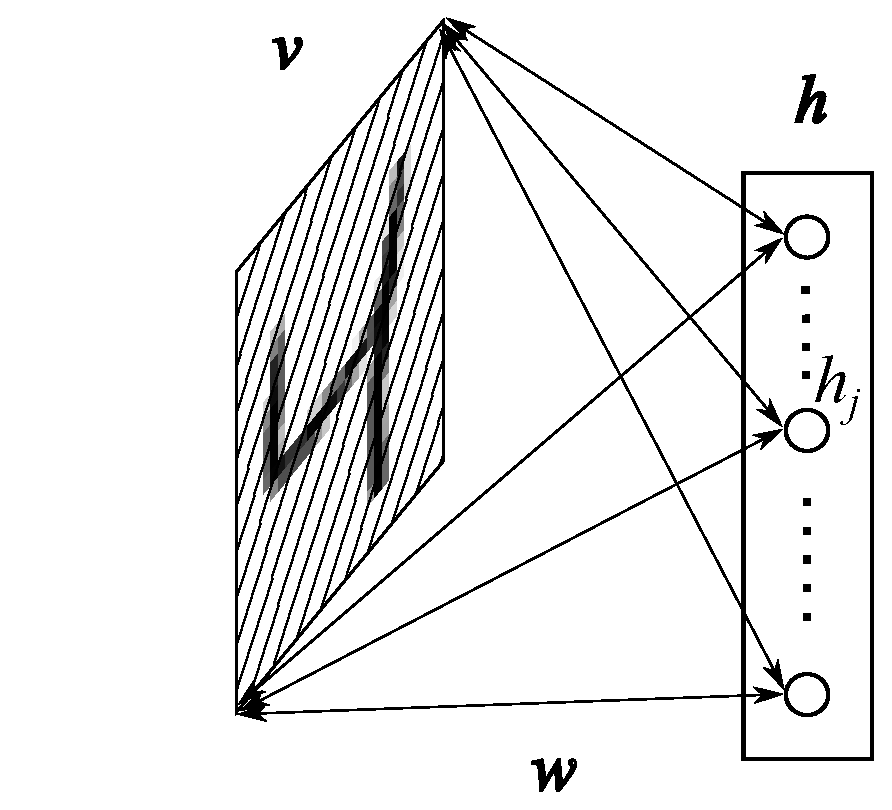
\includegraphics[width=0.8\columnwidth]{lookall_network_v7.eps}
  \caption{実験1のRBM}
  \label{cap:lookall_network}
\end{minipage}
\begin{minipage}{0.45\columnwidth}
  \centering
  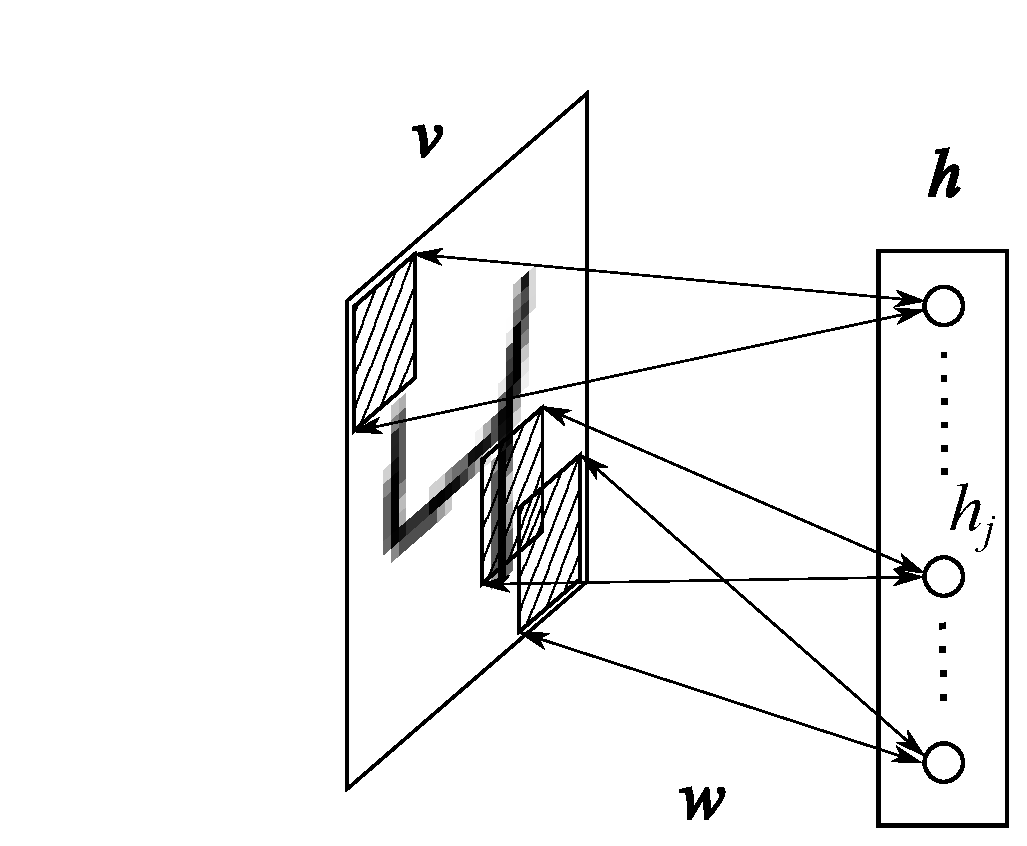
\includegraphics[width=0.9\columnwidth]{lookpartial_network_v8.eps}
  \caption{実験2のRBM}
  \label{cap:lookpartial_network}
\end{minipage}
\end{figure}
\subsubsection{実験1}
%\subsubsection{隠れ層1の素子と可視層の素子が全て結合しているRBM}
図~\ref{cap:lookall_network}のような,
可視層が$784$次元,隠れ層が$500$次元のRBMにて
手書き文字2000枚を用いて
学習率$0.001$で$1000$回の学習をした.
隠れ層の素子${h_j}$は,図~\ref{cap:lookall_network}の斜線で示した
可視層の素子$v_i$すべてと結合している.
\begin{table}%[htb]
\begin{center}
  \caption{各実験における正答率}
  \label{tab:result}
  \begin{tabular}{cccc}
    \hline
    実験   & Training set & Test set\\
    \hline \hline
    実験1  & 89.08\%      & 88.69\% \\
    実験2  & 87.34\%      & 88.36\% \\
    実験3  & 91.86\%      & 91.55\% \\
    \hline
  \end{tabular}
\end{center}
\end{table}

  % 結果
%\input{summary}  % 要約


%%%% 参考文献 %%%

\section{参考文献の書き方}
参考文献は,
本文中で必ず引用する\cite{ohtsuki2008a}.
本文で引用していないものを
参考文献のリストには記述しない\cite{amari89a,radford2015a}.

\bibliographystyle{jabbrv}
% \bibliographystyle{sieicej}
\bibliography{irl_bibs_2017.bib}

\end{document}
